\section{Optimasi dan Penjadwalan Instruksi}

Tahap akhir dari pembangkitan kode adalah memastikan instruksi berjalan seefisien mungkin pada perangkat keras yang memiliki \textit{pipeline}.

\subsection{Penjadwalan Instruksi (Instruction Scheduling)}
CPU modern mengeksekusi instruksi dalam beberapa tahap (\textit{fetch, decode, execute, write-back}). Jika sebuah instruksi membutuhkan hasil dari instruksi sebelumnya yang belum selesai, terjadi hambatan yang disebut \textit{stall} atau \textit{bubble}. \compiler{Instruction Scheduling} berupaya menukar urutan instruksi agar \textit{stall} terminimalisir.

\subsection{Bahaya Jalur Pipa (Pipeline Hazards)}
Kompilator harus mendeteksi dan mengatasi tiga jenis \textit{hazard}:
\begin{enumerate}
    \item \textbf{Data Hazard}: Instruksi bergantung pada data dari instruksi sebelumnya (misal: \textit{Read-After-Write}).
    \item \textbf{Control Hazard}: Terjadi saat ada instruksi percabangan (\textit{jump/branch}), di mana CPU tidak tahu instruksi mana yang harus diambil selanjutnya.
    \item \textbf{Structural Hazard}: Dua instruksi mencoba menggunakan sumber daya perangkat keras yang sama (misal: unit \textit{floating point}) secara bersamaan.
\end{enumerate}

\subsection{Peephole Optimization}
Merupakan teknik optimasi lokal yang memindai jendela kecil instruksi (misal: 2-3 instruksi) dan menggantinya dengan urutan yang lebih efisien. Contoh:
\begin{itemize}
    \item \textit{Redundant Load/Store Elimination}: Menghapus \texttt{STORE R1, x} diikuti \texttt{LOAD x, R1}.
    \item \textit{Strength Reduction}: Mengganti \texttt{MUL R1, 8} dengan \texttt{SHL R1, 3}.
    \item \textit{Algebraic Simplification}: Menghapus \texttt{ADD R1, 0}.
\end{itemize}

\begin{figure}[!htbp]
    \centering
    \adjustbox{max width=0.8\textwidth,center}{%
    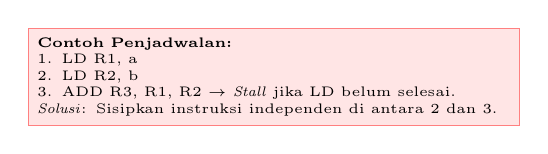
\begin{tikzpicture}[
        rect/.style={rectangle, draw=red!50, fill=red!10, text width=6cm, font=\tiny}
    ]
    \node[rect] (haz) {
        \textbf{Contoh Penjadwalan:}\\
        1. LD R1, a  \\
        2. LD R2, b  \\
        3. ADD R3, R1, R2 $\rightarrow$ \textit{Stall} jika LD belum selesai.\\
        \textit{Solusi}: Sisipkan instruksi independen di antara 2 dan 3.
    };
    \end{tikzpicture}%
    }
    \caption{Ilustrasi Penghindaran Pipeline Stall lewat Penjadwalan}
\end{figure}
